\chapter{Theory}
This chapter contains the theoretical foundations necessary to understand parts of this thesis. 
The signal processing and neural network preliminaries will be explained.
Further the problem formulations will be represented in a mathematical viewpoint.

%The problems will be described in a mathematical way and each solution concept explained so that it can be understood.

% sp
% --
% signal processing

\section{Signal Processing and Feature Extraction}\label{sec:features}
This section describes how raw waveforms from audio files are processed and what meaningfull features can be extracted from them.
\subsection{Raw Audio Waveforms}
Acoustic waves can be recorded by microphones...
\subsection{Spectral Features}
Spectogram
% --
% mfcc

\subsection{Mel Frequency Coefficients}\label{sec:mfcc}
Most commonly the Mel Frequency Cepstral Coefficients (MFCC) are used as input features for Neural Network classifications tasks of audio data.
It is described why they are good features and how they can be visualized to understand them better.

\subsubsection{About Mel Frequency Cepstral Coefficients}
To comprehend the success of the wide use of MFCCs features in Neural Networks and other machine learning applications, it is necessary to understand its processing scheme, which is roughly as following: 
Raw input data is transformed into the frequency domain with an STFT, the power spectrum of this STFT is then segmented into a filter bank with equidistant mel frequencies, then logarithmic scaling is done and as last step a decorrelation with the DCT transform.
Which seem quite complicated at the beginning, is in fact nothing else but some reasonable steps of data compression. 
It is also possible to input a spectrum to the Neural Network, but the amount of input data is just too much.
That is why frequencies are put in certain bands through a filter bank and further decorrelated with a method like the DCT.

\subsubsection{MFCC Feature Usage and Enhancement}
After the MFCCs are computed, they can be used as input features for Neural Networks. 
The important Question here is whether an feature enhancement can be done and if all those computed features are necessarily and meaningful for the training and evaluation success of Neural Networks. Usually not all MFCC coefficients are used as inputs, this is merely done to reduce the computational cost in case the accuracy does not suffer from it.
A good application is to compute 32 MFCC features (with 32 equidistant Mel filter bands) and use only the first 12 of them as inputs.
Further it is also possible to compute derivatives (in the time domain) of MFCC features, denoted as Deltas. 
Those derivatives are simple computed as frame difference of the MFCCs.
A second derivative of MFCC features, known as Double Deltas, are then the frame differences of the Deltas.
At last an energy feature can be computed from each of the MFCCs, Deltas and Double Deltas, each by its own and added to the feature vectors.
Those feature vectors can then be simply stacked at top of each other and used as feature inputs.
In this thesis the feature vectors are stacked as following:
\begin{enumerate}
    \item 12 MFCCs
    \item 1 Energy feature of the 12 MFCCs
    \item 12 Deltas
    \item 1 Energy feature of the 12 Deltas
    \item 12 Double Deltas
    \item 1 Energy feature of the 12 Double Deltas
\end{enumerate}
Which sums up to a 39-dimensional feature vector.

\subsubsection{Visualisation of MFCC features}
A good visualisation of MFCC features is the best way to understand them.
With this thought in mind, much time was spent to create a fitting visual representation of the MFCC features, but this was not an easy task.
MFCCs are not well intended for visualisations, since their individual coefficients value space, can be strongly different from each other.
For example, the first coefficient equals a summation of all filter bands and is therefore some kind of energy measure over all bands, while the other coefficients are weighted sum combinations of the filter bands.
This alone yields in totally different value spaces and value spaces should not differ that much, when features should be represented with colors.
Further it is to mention, that most of the signal energy will be in the lower frequency bands, which also impacts the value space of the individual coefficients a lot.
To show this difference in value space in a negative example in practise, the MFCCs of the self-recorded speech command waveform \enquote{left0.wav} is shown in \rfig{left0_mfcc_only}.

\begin{figure}[!ht]
  \centering
    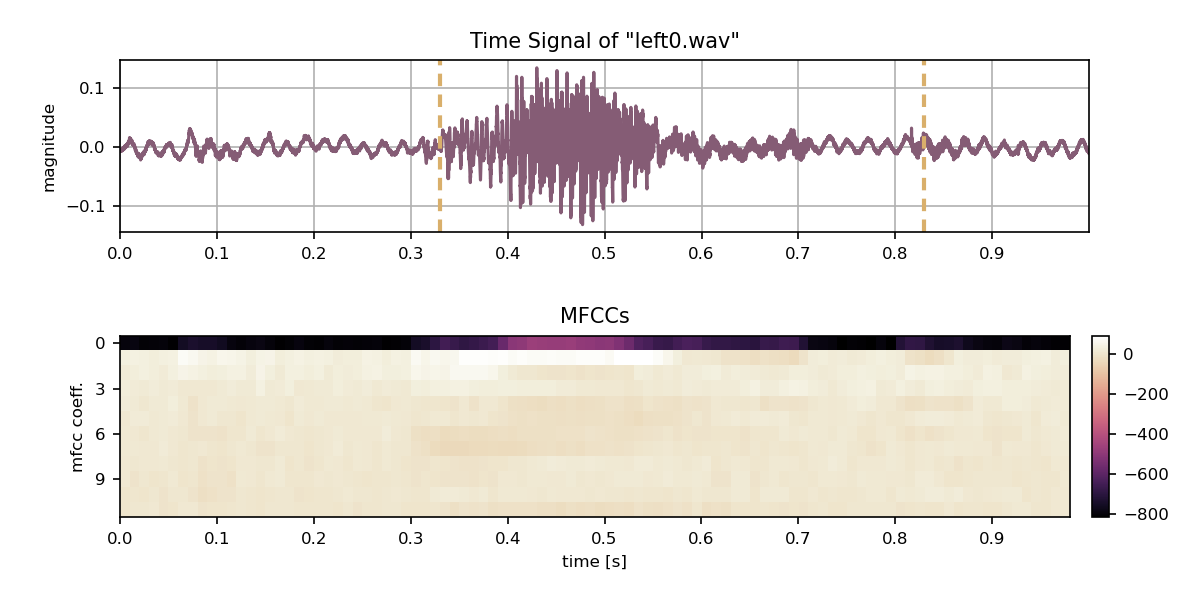
\includegraphics[width=0.75\textwidth]{./3_theory/figs/a3_mfcc/left0_mfcc_only.png}
  \caption{Bad visualisation of the 12 MFCCs features extracted from \enquote{left0.wav}.}
  \label{fig:left0_mfcc_only}
\end{figure}
\FloatBarrier
\noindent
Not much structure of the MFCCs can be seen here, due to the vast value difference of the first coefficient. At least the first coefficient shows, where the center of signal energy is placed on the time scale, but other than that, this visualisation is worthless.
Another very bad visualisation is shown by computing the 39 MFCC feature vectors (with Deltas, Double Deltas and Energies) in \rfig{left0_no_order}.

\begin{figure}[!ht]
  \centering
    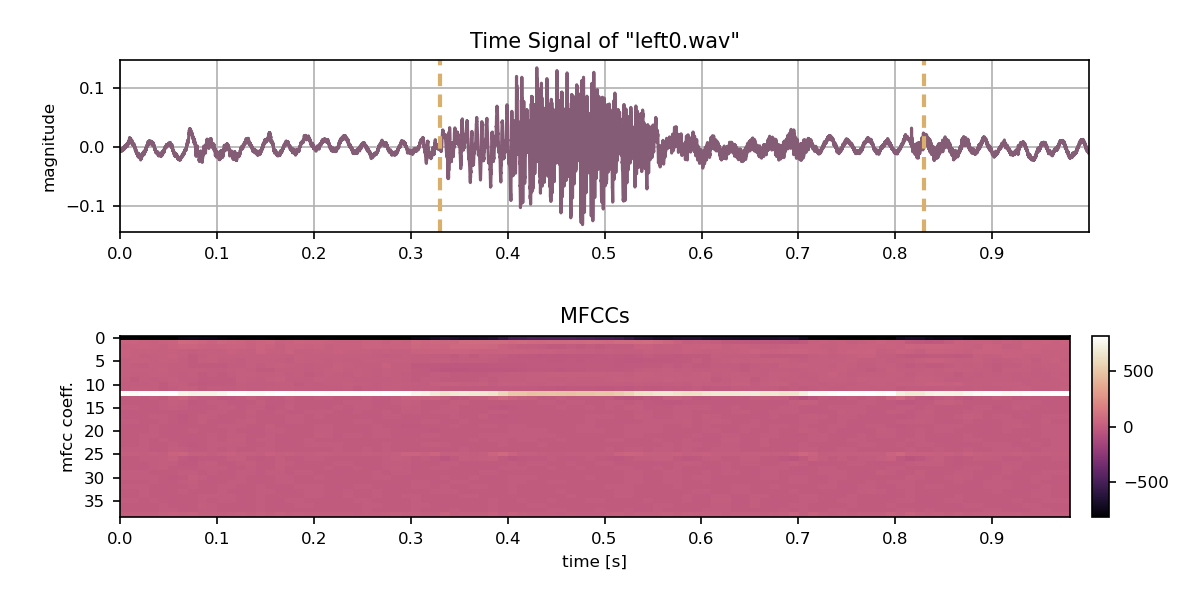
\includegraphics[width=0.75\textwidth]{./3_theory/figs/a3_mfcc/left0_no_order_norm0.png}
  \caption{Very bad visualisation of 39 MFCC features extracted from \enquote{left0.wav}.}
  \label{fig:left0_no_order}
\end{figure}
\FloatBarrier
\noindent
There appears an even greater gap of different value spaces and even less is seen.
One very easy solution is to show the features in different value groups. For instance the first coefficient and its deltas is in one group, the other coefficients in another and the deltas and energies are separated as well in own groups. Now we actually can see some structure in the visualisations, shown in \rfig{left0_order}.

\begin{figure}[!ht]
  \centering
    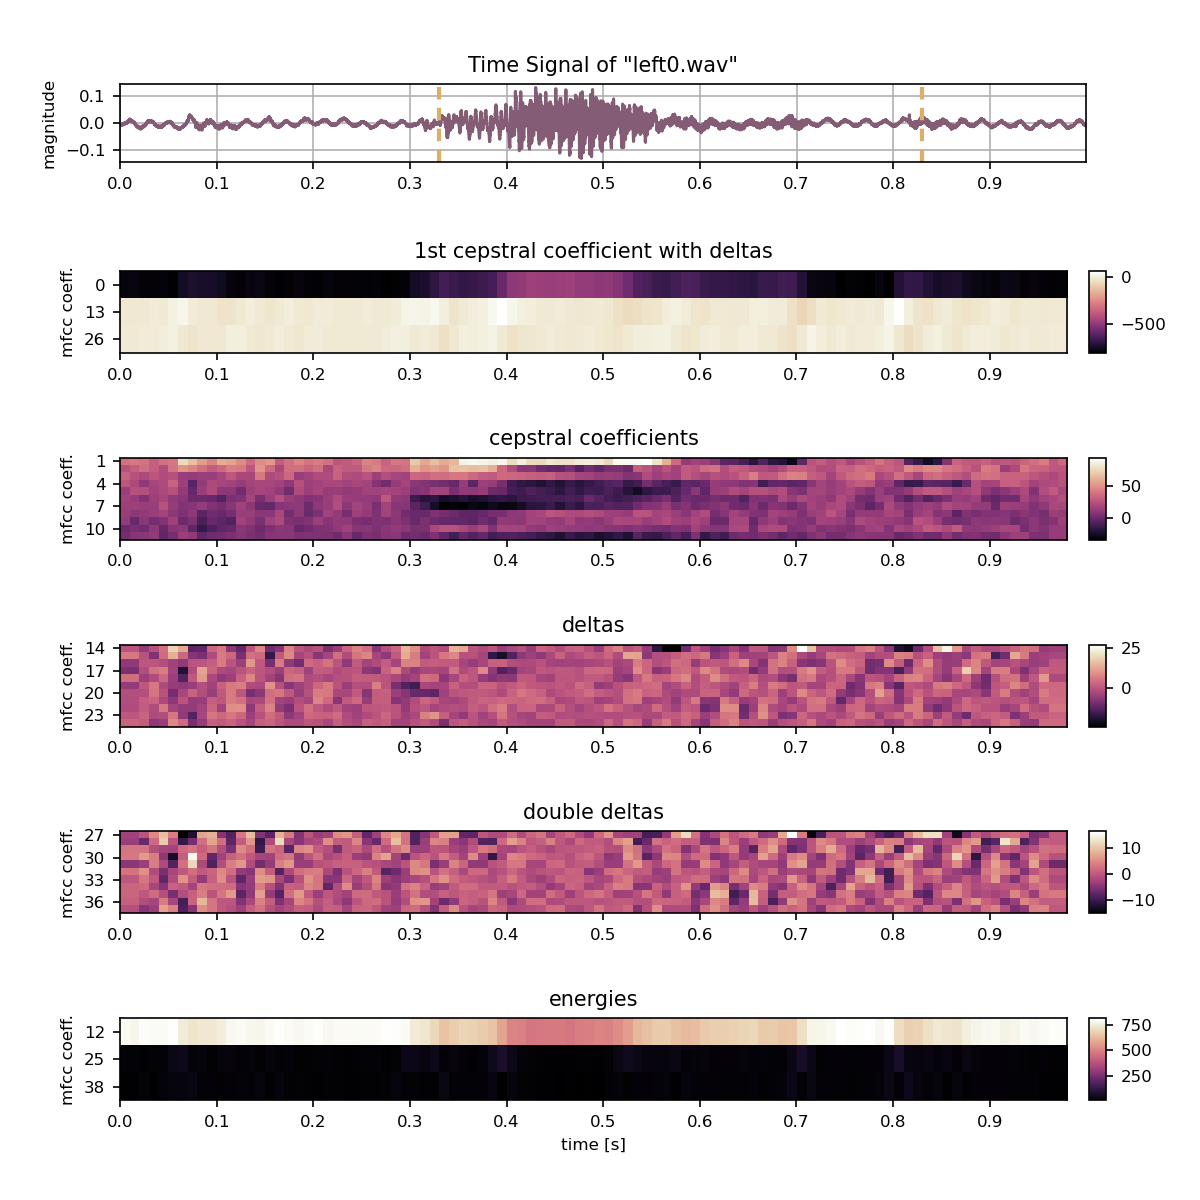
\includegraphics[width=0.75\textwidth]{./3_theory/figs/a3_mfcc/left0_norm0.png}
  \caption{Good visualisation of 39 MFCC features extracted from \enquote{left0.wav} with own value groupings.}
  \label{fig:left0_order}
\end{figure}
\FloatBarrier
\noindent
Another way to improve the visualisation is to normalize the feature vectors over their each own frame dimension with the infinity norm. This will yield a value space of $[0, 1]$ for each feature vector. With this, the visualisation of the 39 MFCC of \enquote{left0.wav} is shown in \rfig{left0_order},

\begin{figure}[!ht]
  \centering
    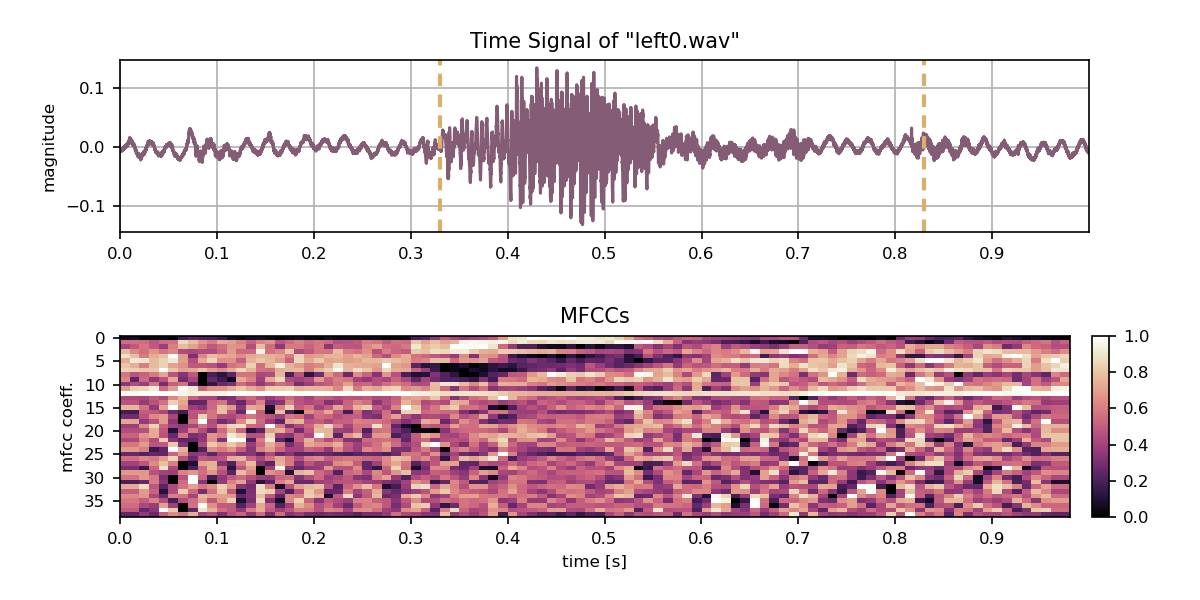
\includegraphics[width=0.75\textwidth]{./3_theory/figs/a3_mfcc/left0_no_order_norm1.png}
  \caption{Normalisation of 39 MFCC features extracted from \enquote{left0.wav}.}
  \label{fig:left0_no_order_norm1}
\end{figure}
\FloatBarrier
\noindent
or in an even better one shown in \rfig{left0_order_norm1}.

\begin{figure}[!ht]
  \centering
    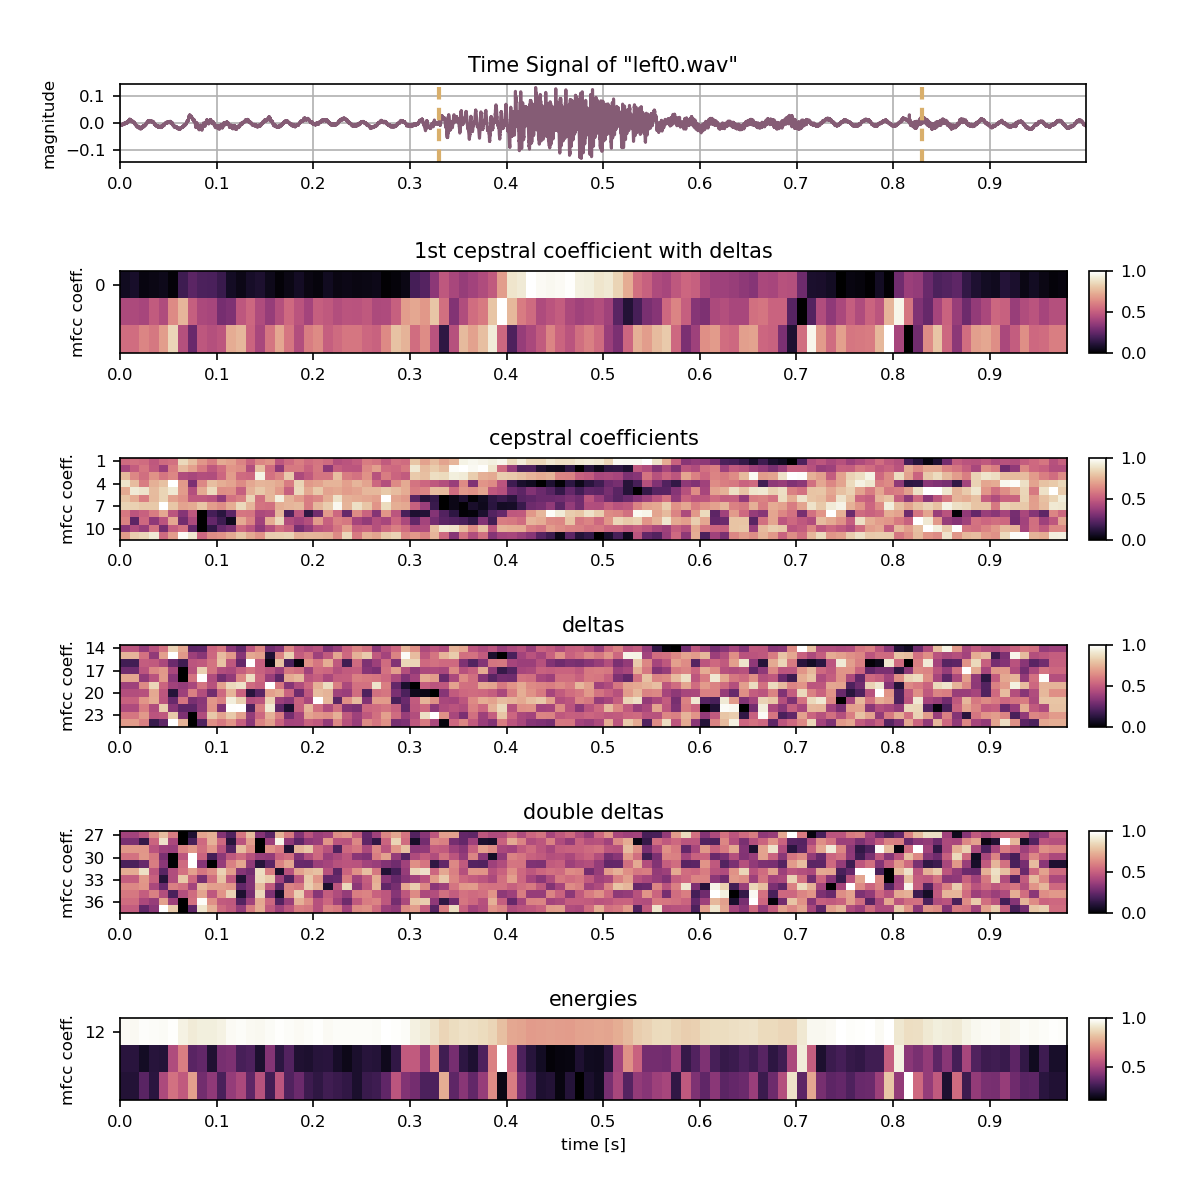
\includegraphics[width=0.75\textwidth]{./3_theory/figs/a3_mfcc/left0_order_norm1.png}
  \caption{Normalisation of 39 MFCC features extracted from \enquote{left0.wav} with groups.}
  \label{fig:left0_order_norm1}
\end{figure}
\FloatBarrier
\noindent
As conclusion, the normalisation in the frame space is an interesting aspect to improve the visualisation of the MFCC features, 
specifically for the cepstral coefficients and the energy features (not the deltas).
Exactly this nice representation was motivating to explore normalisation of feature for Neural Network inputs.
However this is a very crucial thing to do. A normalisation relatives important structures within the feature space and it cannot really be answered if this is a good thing or not.
One more research question arises here: Is it possible to use normalisation for the features as inputs to Neural Networks and what are the results to the accuracy and training of the models.


% ml
\section{Machine Learning Theory}
theory...
\subsection{Neural Network Architectures}\label{sec:nn_arch}
All Neural Network Architectures evaluated within this thesis are presented here.
There will be a general classification between Neural Network Architectures by Convolutional Neural Networks, Adversarial Neural Networks ...
The classification of Convolutional Neural Networks are all Architectures consisting of at least one convolutional layer and the intention to simply classify the speech commands.
As Adversarial Neural Networks we consider Architectures with at least two separate Neural Network Architectures, e.g. a Discriminator and a Generator Network, with the intention to outperform the other Network in a task where they both play a game against each other.
The word game here, is used in the sense of Game Theory, where the goal is to find an equilibrium state where both players are equally satisfied with the state.

% game
\section{Video Game}
Theory?
